\documentclass[11pt]{article}
\usepackage{amsmath,amssymb,amsthm,bbm}
\usepackage{tkz-berge}
\usepackage{tikz,float}
\usepackage{hyperref}
\DeclareMathOperator*{\E}{\mathbb{E}}

\newcommand{\handout}[5]{
  \noindent
  \begin{center}
  \framebox{
    \vbox{
      \hbox to 5.78in { {\bf CIS5200: Machine Learning } \hfill #2 }
      \vspace{4mm}
      \hbox to 5.78in { {\Large \hfill #5  \hfill} }
      \vspace{2mm}
      \hbox to 5.78in { {\em #3 \hfill #4} }
    }
  }
  \end{center}
  \vspace*{4mm}
}

\newcommand{\lecture}[4]{\handout{#1}{#2}{Release Date: #3}{Due Date: #4}{Homework #1}}

% 1-inch margins, from fullpage.sty by H.Partl, Version 2, Dec. 15, 1988.
\topmargin 0pt
\advance \topmargin by -\headheight
\advance \topmargin by -\headsep
\textheight 8.9in
\oddsidemargin 0pt
\evensidemargin \oddsidemargin
\marginparwidth 0.5in
\textwidth 6.5in

\parindent 0in
\parskip 1.5ex

\begin{document}

\lecture{0}{Spring 2023}{January 12, 2023}{January 20, 2023}

% --------------------------------------------------------------
%                         Start here
% --------------------------------------------------------------


{\bf Name: }  Qihang Dai\\

{\bf PennKey:} ahgdyycc\\

{\bf PennID:} 78803164\\

Note: This document is a read-only file. To create an editable version click on Menu in the top left corner of your screen and choose the Copy Project option. 
\section{Written Questions}

\paragraph{A1} 
\begin{enumerate}
    \item  False. 
    \item  False.
    \item  False. $(AB)^T$ = $B^TA^T$
    \item  True. 
\end{enumerate}

\paragraph{A2}
\begin{enumerate}
    \item rank = 2
    \item min span is [1, 2, 3] [0, -3, -2]
\end{enumerate}

\paragraph{A3}
\begin{enumerate}
    \item $det(A - \lambda I) = 0$ $\lambda_1 = 6$ $v_1 = [1, 1, 1]$, and two more eigenvalues
    \item No. it have negative eigenvalue
    \item $\lambda_1 = 6a + 1$ $v_1 = [1, 1, 1]$ 
    \item $\lambda^2 = 36$
\end{enumerate}

\paragraph{A4} 
\begin{enumerate} 
    \item $w$
    \item $-2(y - w^T x) * w$
    \item $ -y * w * ( exp(-yw^T x) / (1 + exp(-yw^T x)) )$
    \item $2Ax$
\end{enumerate}

\paragraph{A5}
\begin{enumerate}
    \item b = 0
    \item $\text{distance} = \frac{|w^\intercal x_0 + b|}{\left|w\right|}$
\end{enumerate}

\paragraph{A6} 
\begin{enumerate}
    \item true
    \item true
    \item false
    \item true
\end{enumerate}

\paragraph{A7} 
\begin{enumerate}
    \item No. the hessian is not positive semi-definite
    \item x1, x2 all equals to 0, or x1 = 0 $x_2$ = $\pm \sqrt{\frac{1}{2}}$
    \item -3/8 
\end{enumerate}

\paragraph{A8}

solved by Bayes rule
$$ P(sunny/forcastSunny) = \frac{P(forcastSunny/sunny) * P(sunny)}{P(forcastSunny)} $$
$$ P(sunny) = 0.1, P(-sunny) = 0.9$$
$$P(-for/sunny) = 0.15, P(for/sunny) = 1 - P(-f/s) = 0.85, P(f/-s) = 0.05$$
$$P(for) = P(f/s) * P(s) + P(f/-s) * P(-s) = 0.85 * 0.1 + 0.05 * 0.9 = 0.13$$
$$P(sunny/for) = \frac{P(for/s) * P(s)}{P(for)} = \frac{0.85 * 0.1}{0.13} = 0.65$$

\paragraph{A9} 
\begin{enumerate}
    \item $a = \frac{1}{\sigma}$ $b = -\frac{\mu}{\sigma}$
    \item $E[z^2] = var(z) + (E[z])^2 = \sigma^2 + \mu^2$
    \item $N(\mu + \bar \mu, \sigma^2 + \bar \sigma^2)$
\end{enumerate}

\paragraph{A10} 
\begin{enumerate}
    \item 1/p
    \item independent event, so also p
\end{enumerate}

\end{document}
\section{Python Programming Questions}

% Complete questions in your iPython notebook and place all results here.

% TODO: add matplotlib plot (Q4) here
TODO : Please add the matplotlib plot for Q4 below
\begin{figure}
  \centering
  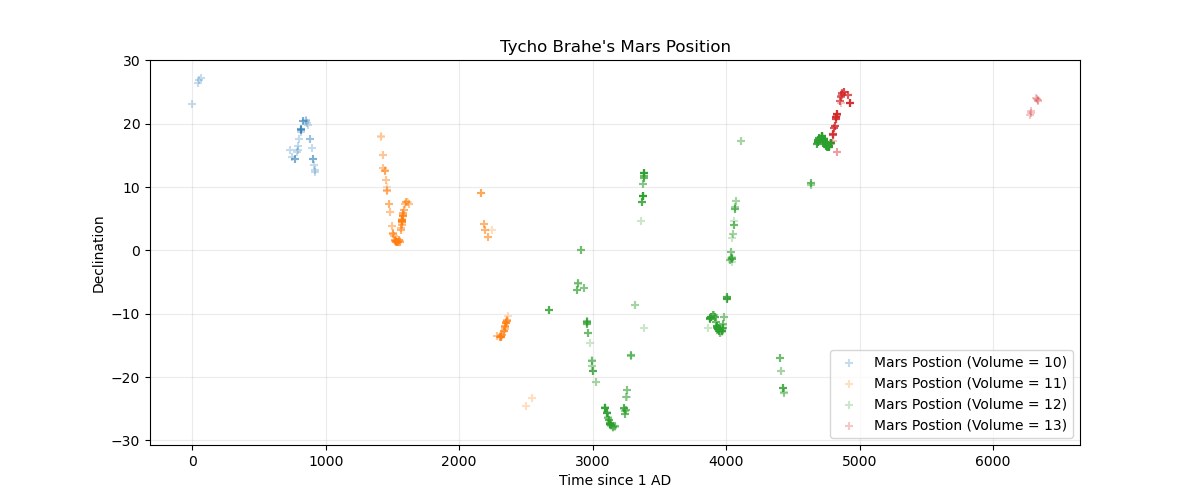
\includegraphics[width=0.8\textwidth]{example-figure.png}
  \caption{Figure for Q4 (MatplotLib)}
\end{figure}

\end{document} 